\section{Catalogo de estrelas}
\label{sec:catalogo_de_estrelas}

A criação do catálogo é realizada por satélites especialmente criados e lançados com este propósito, como o é o caso do NASA I/239, que compõem o banco de dados do Hipparcos and Tycho. Este banco de dados é encontrado em ~\cite[]{ESA}.

O banco de dados possui uma tabela principal de informações, com o formato mostrado na Figura ~\ref{fig:Resumo_impetracao_parte_esquerda_Hipparcos}.

\begin{figure}[H]
	\centering
	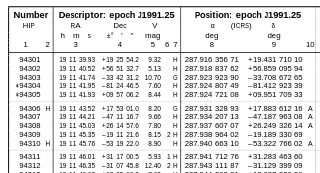
\includegraphics[width=.7\columnwidth]{images/Resumo_impetracao_parte_esquerda_Hipparcos.png}
	\caption{Resumo de impetração da parte esquerda do catálogo Hipparcos. Fonte: ~\cite[]{ESA}}
	\label{fig:Resumo_impetracao_parte_esquerda_Hipparcos}
\end{figure}

Essa tabela possui muitas informações que não serão utilizadas, incluindo uma quantidade de estrela muito grande, 
portanto o banco de dados foi filtrado com apenas alguns campos de dados restantes, número de catalogação, ascensão reta (em °), 
declinação (em °) e magnitude, que mostrado na Figura ~\ref{fig:Caracteristicas_matriz}. 
Além disto foi realizado uma filtragem por estrelas com magnitude cinco ou inferior, 
o que significa que apenas as estrelas mais brilhantes permaneceram na base de dados do sistema. 
Para a visualização das estrelas restantes utiliza-se o sistema equatorial de coordenadas, resultando nos plots apresentados nas figuras ~\ref{fig:Rrepresentacao_2D} e \ref{fig:Representacao_3D}.

\begin{figure}[H]
	\centering
	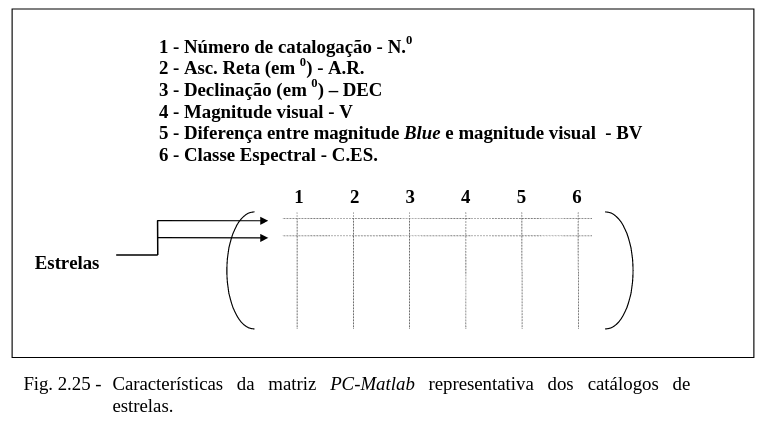
\includegraphics[width=.7\columnwidth, trim={0 60 0 0}, clip]{images/Caracteristicas_matriz.png}
	\caption{Características de matriz representativa do catálogo estelar. Fonte: ~\cite[]{Carvalho}}
	\label{fig:Caracteristicas_matriz}
\end{figure}

\begin{figure}[H]
	\centering
	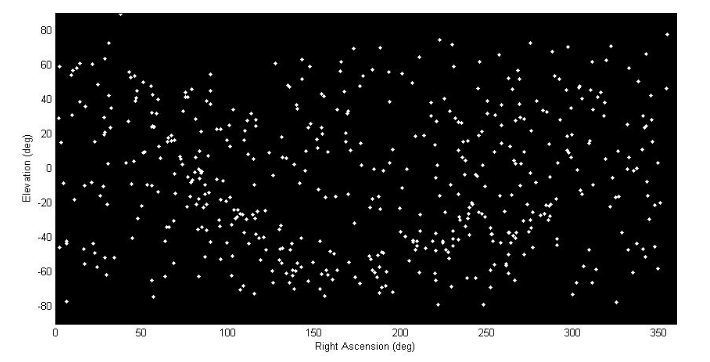
\includegraphics[width=.7\columnwidth]{images/Rrepresentacao_2D.png}
	\caption{Catálogo estelar representação em 2D. Fonte: ~\cite[]{Diaz}}
	\label{fig:Rrepresentacao_2D}
\end{figure}

\begin{figure}[H]
	\centering
	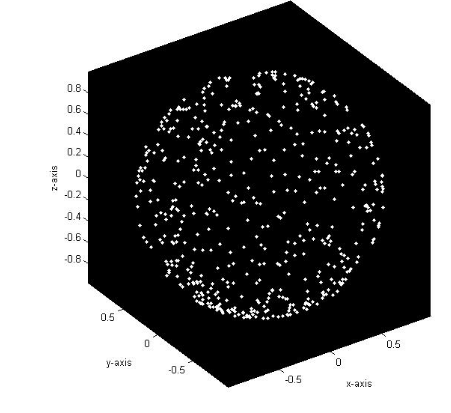
\includegraphics[width=.7\columnwidth]{images/Representacao_3D.png}
	\caption{Catálogo estelar representação em 3D. Fonte: ~\cite[]{Diaz}}
	\label{fig:Representacao_3D}
\end{figure}

